\documentclass[]{beamer}
% Class options include: notes, notesonly, handout, trans,
%                        hidesubsections, shadesubsections,
%                        inrow, blue, red, grey, brown

% Theme for beamer presentation.
\usepackage{tabularx}
\usepackage{graphicx}
\usepackage[export]{adjustbox}
\usepackage{beamerthemesplit} 
% Other themes include: beamerthemebars, beamerthemelined, 
%                       beamerthemetree, beamerthemetreebars  

%\usepackage{beamerthemebars}

\title{PyGame- SDES Battle}    % Enter your title between curly braces
\author{Aman Khanna (133070052),\\
Amit Chawla (133070044),\\
Shaishav Shah (133070050)
}                 % Enter your name between curly braces
\institute{
IIT Bombay}      % Enter your institute name between curly braces
\date{\today}                    % Enter the date or \today between curly braces
\setbeamertemplate{footline}
{
    \leavevmode%
    \hbox{%
        \begin{beamercolorbox}[wd=.75\paperwidth,ht=3ex,dp=1ex,center]{author in head/foot}%
            \usebeamerfont{author in head/foot}\insertshortauthor
        \end{beamercolorbox}%
        \begin{beamercolorbox}[wd=.25\paperwidth,ht=3ex,dp=1ex,center]{title in head/foot}%
            \usebeamerfont{title in head/foot}\insertshorttitle
        \end{beamercolorbox}%
        }%
        \vskip0pt%
    }


\begin{document}

% Creates title page of slide show using above information
\begin{frame}
  \titlepage
  \begin{center}
      Project Group No: 6\\
      github code link: \url{https://github.com/amankhanna89/ae_663_project}
  \end{center}

\end{frame}
\note{Talk for 2 minutes} % Add notes to yourself that will be displayed when
                           % typeset with the notes or notesonly class options


\begin{frame}
  \frametitle{Introduction}
  \begin{center}
  \begin{itemize}
    \item We  are making a game in python : \textbf{\textit{SDES Battle}} using pygame library.
    \item multiple stages in which obstacles(examinations and assignments)
 are appearing in screen- move from Right to Left- starting at random position
    \item Player (student) has to tackle them by firing.
    \item Score obtained will be displayed on top-right.
    \item After completion of each stage, notification window will be appeared.
  \end{itemize}
   
  \end{center}

  
  \end{frame}


% Creates table of contents slide incorporating
% all \section and \subsection commands
\begin{frame}
  \frametitle{Features}
    \begin{center}
  \begin{itemize}
    \item Upon user input (Clicking on \textit{Begin}), the game will start.
    \item Obstacles of different shape will move from right to left. 
    \item Player has to fire to destruct these obstacles.
    \item If fire passes within the dimension, of obstacles, destruct the object 
	and display the score on the top
    \item If any obstacle is missed, reduce the number of attempts (initially, the attempts=3) 
    \item If the attempts are over, Display \textit{Game Over}
    \item As the stage progresses, 
    \begin{enumerate}
     \item The speed of the obstacle increases.
     \item The background changes, and its speed also increases.
     \item Minimum threshold score required to clear the level increases. 
    \end{enumerate}
   \item After completion of stage each stage, message will be displayed on the screen.
    
  \end{itemize}
   
  \end{center}
\end{frame}



\begin{frame}
  \frametitle{Libraries used and their Features}
  \begin {itemize}
   \item pygame
   \begin {enumerate}
    \item Initialize all the gaming features: display, background
    \item Includes sound effects.
    \item Continuously scan the keyboard and take action accordingly.
    
   \end {enumerate}
   \item xlib
   \begin {enumerate}
    \item 
   \end {enumerate}
   \item serge
   \begin {enumerate}
    \item 
   \end {enumerate}
    \item os
    \item sys
    \item math
    \item subprocess
  \end {itemize}


  \end{frame}


\begin{frame}
  \frametitle{Programming Efforts}
  \begin {itemize}
   \item Initialize all the global variables.
   \item Initialize all the local variables upon function call: reset
   \item Initialize gaming window using pygame modules
   \item background image initialization and movement using 
    continuously shifting of images.
   \item Fire object:
   \begin {enumerate}
    \item Define a class called \textit{make\_fire}. %The class itself is self explanatory. 
    \item Define different parameters for fires, sucha as shape, color, speed
    \item Construct the fire object when fire-key is pressed.
    \item Destruct the fire object when target is destroyed or the fire reaches to right end.
   \end {enumerate}
    
   \end {itemize}


  \end{frame}


\begin{frame}
  \frametitle{Programming Efforts (contd.)}
  \begin {itemize}
   \item Target object:
   \begin {enumerate}
    \item Define a class called \textit{make\_target}. %The class itself is self explanatory. 
    \item Define different parameters for targets, sucha as images,
      score,
    \item Construct the target object randomly and in random number on the screen.
    \item Take multiple image for each target so that it seems moving.
    \item Destruct the target object when its co-ordinate matches with fire
	or the target reaches to left end.
    \item if the object is destructed through fire, increase the score
	equal to member score for that object.
	
   \end {enumerate}
   
   \item Key pressing and functioning
   \item Player movement
    \begin {enumerate}
     \item 
    \end {enumerate}
    \item fire object is generated with its position same as player position
	when fire key is pressed.
    
   
  \end {itemize}


  \end{frame}
  
  

\begin{frame}
  \frametitle{Keys Functioning}

  \end{frame}

  
  
\begin{frame}
  \frametitle{Demo}

  \end{frame}

  
  
\begin{frame}
  \frametitle{Work Done}
  \begin{center}
  \begin{columns}[c]
  \column{2.3in}
    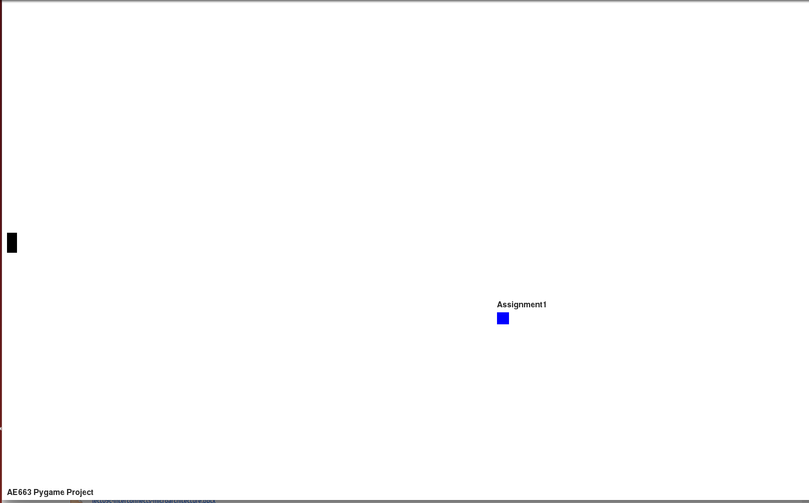
\includegraphics[scale=0.21, frame]{./diagram/rsz_screen_01}\\
    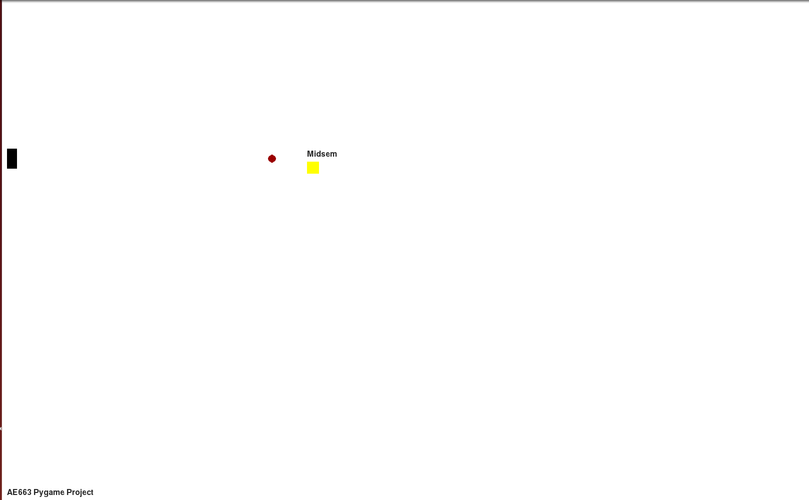
\includegraphics[scale=0.21,  frame]{./diagram/rsz_screen_03}
  \column{2.3in}
  %\begin{center}
  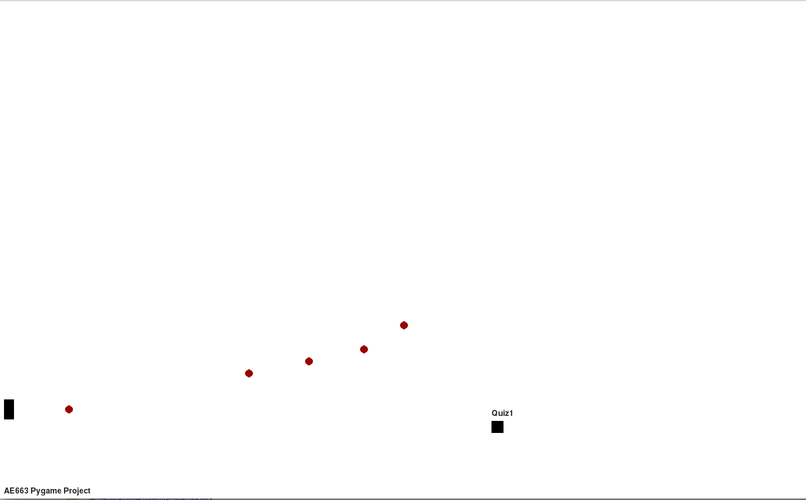
\includegraphics[scale=0.21, frame]{./diagram/rsz_screen_02}\\
  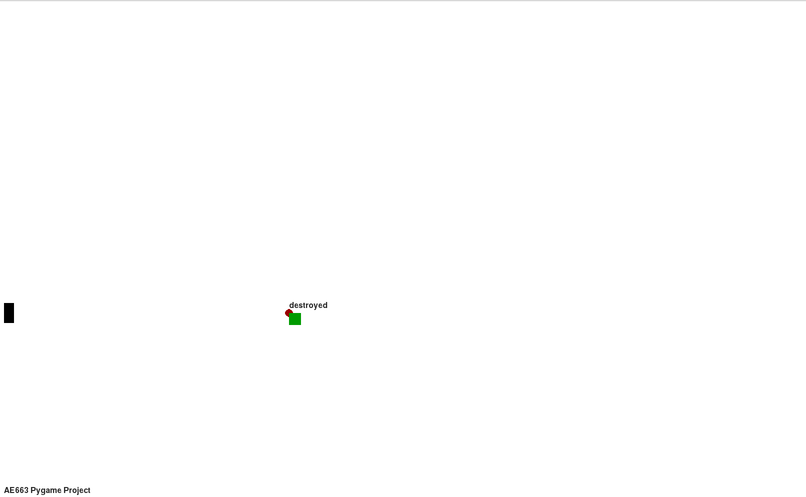
\includegraphics[scale=0.21,  frame]{./diagram/rsz_screen_04}
  %\end{center}
  \end {columns}
   
  \end{center}

  
  \end{frame}

\begin{frame}
  \frametitle{Future Work (Depending on time permit)}
  \begin{center}
    \begin{itemize}
    \item Graphics movement on the background
    \item Complex firing can be made by making player static and firing at different angles.
    \item Add sound for firing and obstacle destruction.
    \end{itemize}
  \end{center}
\end{frame}





\end {document}
